\vspace{0.5 cm}
\textcolor{blue} {\textit{Elouan AUTRET}}
\vspace{0.3 cm}
\subsection{Thick Functions}

A thick function is a function of $\mathbb{R^{\textnormal{\ensuremath{n}}}}$ in $\mathbb{R^{\textnormal{\ensuremath{p}}}}$ that associate to an element x $\in \mathbb{R^{\textnormal{\ensuremath{n}}}}$ a convex element of $\mathbb{R^{\textnormal{\ensuremath{p}}}}$ where there can have intervals as parameters of the function.

For example, consider the function f :
\begin{algorithmic}[H]
\STATE f :  $\mathbb{R} \rightarrow \mathbb{R} $
\STATE $\mathbf{x} \rightarrow \mathbf{x}+ \mathbb{[ \,\textnormal{1},\textnormal{2}] \,}$
\end{algorithmic}

If the width of x is null (ex: [1,1]) the width of f(x) will be strictly greater than zero ([2,3]) (see figure~\ref{fig:thickFunction}).

A thick function can be consider as an interval of classical function with the same principal properties like an lower bound and an upper bound, [f] is equal to [$f^{\textnormal{\ensuremath{-}}}$,$f^{\textnormal{\ensuremath{+}}}$]  where $f^{\textnormal{\ensuremath{-}}}$ is the lower bound function and $f^{\textnormal{\ensuremath{+}}}$ is the upper one. See the example for  a function from $\mathbb{R} $ in$ \mathbb{R} $ :

\begin{figure}[H]
\centering
    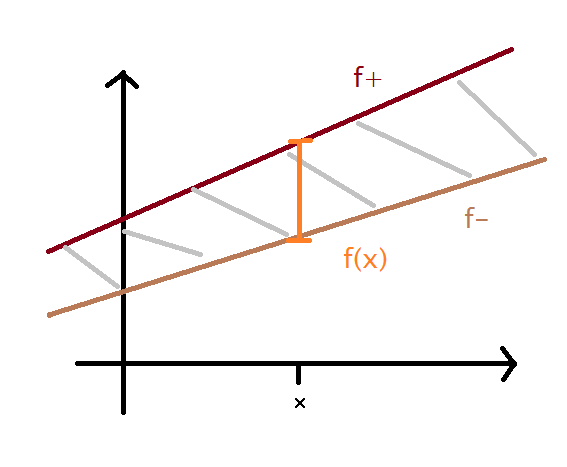
\includegraphics[scale=0.8,angle=0]{thick_function.png}
    \caption{Example of a thick function  $\mathbb{R} \rightarrow \mathbb{R} $.}
    \label{fig:thickFunction}
\end{figure}

Those thick functions allow, for the surveillance problem, the modelling of the uncertainty of
the position of the boat that will watch the bay.\\
Indeed, the position can be given by a GPS but the result is not absolute, the real position can be off by a few meters, for example if [1,2] is the position of the boat and 10 is the range of detection by the boat, then the set of the secure zone without uncertainty would be:

\begin{equation}
 \mathbf{S} = \{ x \in \mathbf{R}^{\textnormal{\ensuremath{2}}} | (x(1)-1)^{\textnormal{\ensuremath{2}}} + (x(2)-2)^{\textnormal{\ensuremath{2}}} \leq 100 \}  \label{eqDIST}
\end{equation}

But if we add an uncertainty of 0.5 to the position then the set become:
\begin{equation}
 \mathbf{S} = \{ x \in \mathbf{R}^{\textnormal{\ensuremath{2}}} | (x(1)-[ \,0.5,1.5] \,)^{\textnormal{\ensuremath{2}}} + (x(2)-[ \,1.5,2.5] \,)^{\textnormal{\ensuremath{2}}} \leq 100 \}  \label{eqDISTTHICK}
 \end{equation}

This set can easily be found with interval analysis using the ibex library with a separator for the precedent equation ~\eqref{eqDIST}, then by proceeding with the SILVIA algorithm and associating the code with VIBES (a viewer tool) the zones reached by the boat can be visualized:

\begin{figure}[H]
\centering
    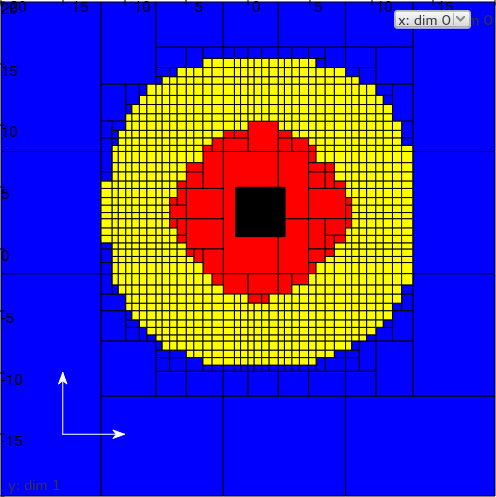
\includegraphics[scale=0.8,angle=0]{1_boat_no_efficient_border.png}
    \caption{Zone secured by one boat in red, yellow zone is uncertain,blue is not secured,the black square are the possible position of the boat.}
    \label{fig:SecureZoneOneBoat}
\end{figure}

The figure~\ref{fig:SecureZoneOneBoat} shows the zone covered by the surveillance boat, in red the zone is certain to be covered, in yellow it is not sure it depends on the real place of the boat in the black square or uncertainty.

\subsection{Test for Biscay Bay Surveillance}
For all this section we consider that for all $\mathbf{X} \in \mathbb{R^{\textnormal{\ensuremath{2}}}}$,  $\mathbf{X}$ is included in the bay of Biscay (the set $\mathbb{G}$) in order to facilitate the comprehension.\\
The figure~\ref{fig:SecureZoneOneBoat} shows that the zone covered by the boats can be found but it also point out that the computing of the zone is not efficient, the uncertain zone cannot be classify as out or in the secured zone so the SIVIA algorithm cut the boxes to their minimal size even if it is possible to know their status of uncertainty thus proceeding to more computation than needed. A new test is required instead of a simple separator to allow a faster and cleaner computation of the secured zone.
The test can be found in the algorithm ~\ref{alg:one_boat_alg} which take a box (an element of $\mathbb{R}^{\textnormal{\ensuremath{2}}}$)) and determine its status, the state can vary between six status where for now the border regroup more or less three status as it can be seen in the following table:

\begin{center}
\begin{tabular}{|m{0.10\linewidth}|m{0.15\linewidth}|m{0.5\linewidth}|}
\hline
 Symbol & In Algorithm  & Meaning  \\ \hline
 0 & OUT & Box is not in the Secure Zone  \\ \hline
 1 & IN & Box is in the secure zone \\ \hline
 ? & UNKNOWN & Box is at the border of the secure zone  \\ \hline
[0,?]& UNKNOWN  & Box is on the external border of the covert zone \\ \hline
[?,1]& UNKNOWN  & Box is on the internal border of the covert zone\\ \hline
[0,1]& MAYBE  & Box is in the uncertainty zone\\ \hline
   
\end{tabular}
\end{center}

The test~\ref{alg:one_boat_alg} need to invert a thick set created by the function in use, here it is the euclidean norm for interval:
 \[ f : \mathbb{R^{\textnormal{\ensuremath{2}}}} \rightarrow \mathbb{R} \]
   \[x \rightarrow \|X-m\|^{\textnormal{\ensuremath{2}}}\]
   
 Where: 
 \[f^{\textnormal{\ensuremath{-}}} = (X[0]-m[0])^{\textnormal{\ensuremath{2}}}+(X[1]-m[1])^{\textnormal{\ensuremath{2}}}\] 
\[f^{\textnormal{\ensuremath{+}}} = max((X[0]-m[0].lb())^{\textnormal{\ensuremath{2}}},(X[0]-m[0].ub())^{\textnormal{\ensuremath{2}}}) + \
                  max((X[1]-m[1].lb())^{\textnormal{\ensuremath{2}}},(X[1]-m[1].ub())^{\textnormal{\ensuremath{2}}})\] 

\begin{algorithm}[H]
\caption{Is $\mathbf{X} \subseteq \mathbb{S}_m$ , $\mathbb{S}_m =$ Secured Zone by boat $m$ and $\mathbf{X} \in \mathbb{R^{\textnormal{\ensuremath{2}}}}$ }
\label{alg:one_boat_alg}
\begin{algorithmic}[1]
\REQUIRE $X$,$range $ (reach of boat),$m$ (position of boat)\\
  $ f : \mathbb{R^{\textnormal{\ensuremath{2}}}} \rightarrow \mathbb{R} $\\
   $x \rightarrow \|X-m\|^{\textnormal{\ensuremath{2}}}$
\STATE $Xm \leftarrow f^{\textnormal{\ensuremath{-}}}(X) $
\STATE $Xp \leftarrow f^{\textnormal{\ensuremath{+}}}(X) $
\STATE $Xub \leftarrow Xp | Xm$
\IF{$Xub \cap \mathbb{[ \,\textnormal{0},\textnormal{range}^{\textnormal{\ensuremath{2}}}] \,} =  \emptyset $}
\RETURN $\textnormal{OUT}$
\ELSIF {$Xub \subseteq \mathbb{[ \,\textnormal{0},\textnormal{range}^{\textnormal{\ensuremath{2}}}] \,} $}
\RETURN $\textnormal{IN}$
\ELSE
\IF{ $\textnormal{range}^{\textnormal{\ensuremath{2}}} - Xp.ub() < \textnormal{0}] $}
\IF{ $Xm - \textnormal{range}^{\textnormal{\ensuremath{2}}} \subseteq \mathbb{[ \,-\infty,\textnormal{0}] \,}$}
\RETURN $\textnormal{MAYBE}$ \label{op1}
\ELSE
\RETURN $\textnormal{UNKNOWN (later:UNKNOWN2)}$ \label{op0}
\ENDIF
\ELSE
\RETURN $\textnormal{UNKNOWN}$
\ENDIF
\ENDIF
\end{algorithmic}
\end{algorithm}

The solution of the zone covered by the boat resemble to the figure~\ref{fig:SecureZoneMAYBEOneBoat}, and by seeing the size of the boxes (there are less boxes) in the uncertain zone it is sure that the computation was efficient:

\begin{figure}[H]
\centering
    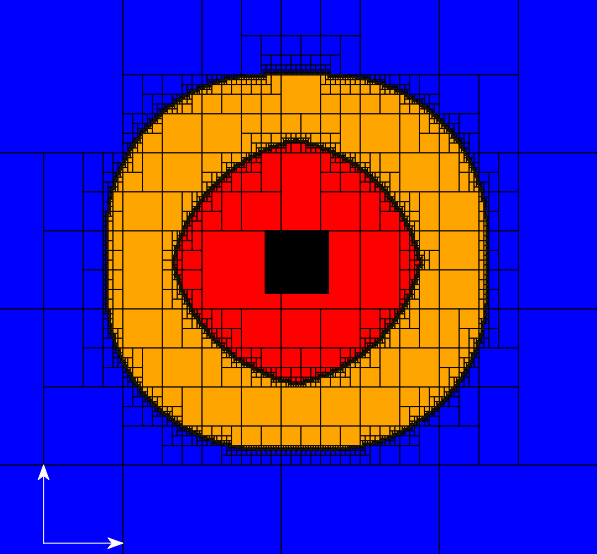
\includegraphics[scale=0.6,angle=0]{1_boat_efficient_border.png}
    \caption{Zone secured by one boat in red, orange zone is uncertain, yellow is the border and blue is not secured.}
    \label{fig:SecureZoneMAYBEOneBoat}
\end{figure}

Now that the algorithm is working for on boat, other can be added:

\begin{figure}[H]
\centering
    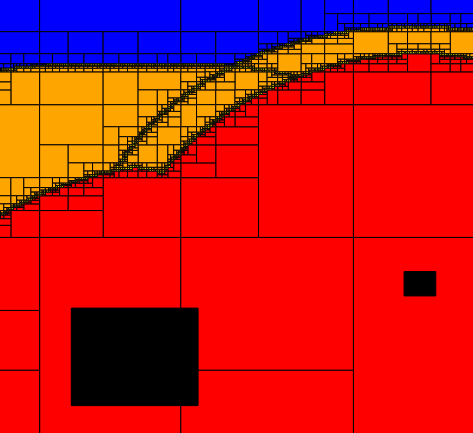
\includegraphics[scale=0.9,angle=0]{2_boat_overwriting_border.png}
    \caption{Zone secured by two boat in red, orange zone is uncertain, yellow is the border.}
    \label{fig:SecureZoneTwoBoat}
\end{figure}


The table shown earlier was not completely correct, as it was omitting the overlapping of the different boats as seen in the figure~\ref{fig:SecureZoneTwoBoat}, the external border of the zone covered by on boat is overlapping the uncertain zone of a different boat.\newline

In order to avoid those wrong and useless computations, the algorithm~\ref{alg:one_boat_alg} need to take into account the fact that an external border for a boat can be in an uncertain zone of an another boat, this change the correspondence table to:

\begin{center}
\begin{tabular}{|m{0.10\linewidth}|m{0.15\linewidth}|m{0.5\linewidth}|}
\hline
 Symbol & In Algorithm  & Meaning  \\ \hline
 0 & OUT & Box is not in the Secure Zone  \\ \hline
 1 & IN & Box is in the secure zone \\ \hline
 ? & UNKNOWN & Box is at the border of the secure zone  \\ \hline
[0,?]& UNKNOWN2  & Box is on the external border of the covert zone \\ \hline
[?,1]& UNKNOWN  & Box is on the internal border of the covert zone\\ \hline
[0,1]& MAYBE  & Box is in the uncertainty zone\\ \hline
   
\end{tabular}
\end{center}

Now the algorithm~\ref{alg:one_boat_alg} need to update this is done by changing the return from UNKNOWN to UNKNOWN2 in operand~\ref{op0}.\\
But the result seen in figure~\ref{fig:SecureZoneTwoBoat} need to fusion result of algorithm~\ref{alg:one_boat_alg} between the different boat,  this can be done by evaluating the result two by two boats, which correspond to the Truth table that follow:

\begin{center}
\begin{tabular}{|m{0.20\linewidth}|m{0.07\linewidth}|m{0.07\linewidth}|m{0.07\linewidth}|m{0.07\linewidth}|m{0.07\linewidth}|m{0.07\linewidth}|}
\hline
Test1/Test2 & 0 & 1 & ? & [0,?] &  [?,1] & [0,1] \\ \hline
          0 & 0 & 1 & ? & [0,?] &  [?,1] & [0,1]  \\ \hline
          1 &   & 1 & 1 &   1   &    1   &   1  \\ \hline
          ? &   &   & ? &   ?   &  [?,1] & [?,1] \\ \hline
      [0,?] &   &   &   & [0,?] &  [?,1] & [0,1] \\ \hline
      [?,1] &   &   &   &       &  [?,1] & [?,1] \\ \hline
      [0,1] &   &   &   &       &        & [0,1]  \\ \hline   
\end{tabular}
\end{center}

This truth table is translated in an algorithm(see~\ref{alg:fus_boat_alg}).

\begin{algorithm}[H]
\caption{Is $\mathbf{X} \subseteq \mathbb{S}$ , $\mathbb{S} =$ Secure Zone and $\mathbf{X} \in \mathbb{R^{\textnormal{\ensuremath{2}}}}$ }
\label{alg:fus_boat_alg}
\begin{algorithmic}[1]
\REQUIRE $X$,$range $ (reach of a boat),$M$ (list of position of boats)
\STATE $R \leftarrow \{\textnormal{Algorithme$~\ref{alg:one_boat_alg}
$(X,range,m)}\}_{m\in M}$
\IF{$\textnormal{IN} \subset R$}
\RETURN $\textnormal{IN}$
\ELSIF {$\textnormal{UNKNOWN} \subset R $}
\RETURN $\textnormal{UNKNOWN}$
\ELSIF {$\textnormal{MAYBE} \subset R $}
\RETURN $\textnormal{MAYBE}$
\ELSIF {$\forall r \in R $, $ r = \textnormal{OUT} $}
\RETURN $\textnormal{OUT}$
\ELSE
\RETURN $\textnormal{UNKNOWN}$
\ENDIF
\end{algorithmic}
\end{algorithm}

\begin{figure}[H]
\centering
    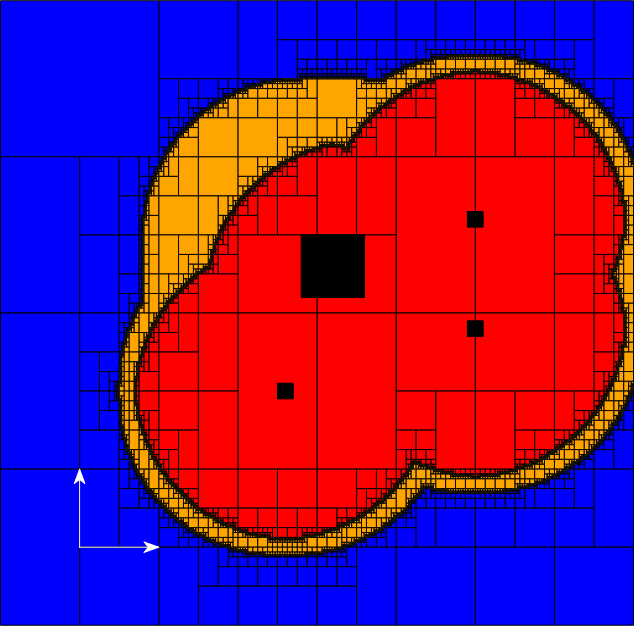
\includegraphics[scale=0.6,angle=0]{4_boat_right_border.png}
    \caption{Zone secured by four boat in red, orange zone is uncertain,blue is not secured.}
    \label{fig:SecureZoneFourBoat}
\end{figure}


Those last changes make the computation of the zone more efficient and correct, in figure~\ref{fig:SecureZoneFourBoat} there is no more overlapping of the external border.\\
If the uncertain zone is not needed the computation of the algorithm SIVIA can be accelerated by ignoring it. This can be done by changing the return value in the operand~\ref{op0} in the algorithm~\ref{alg:one_boat_alg} from UNKNOWN2 to OUT and the return value in the operand~\ref{op1} from MAYBE to OUT (the second change will not improve efficiency but just place the box in the right set), the result can be observed in figure~\ref{fig:SecureZoneFourFastBoat}.

\begin{figure}[H]
\centering
    \begin{minipage}[b]{0.4\textwidth}
    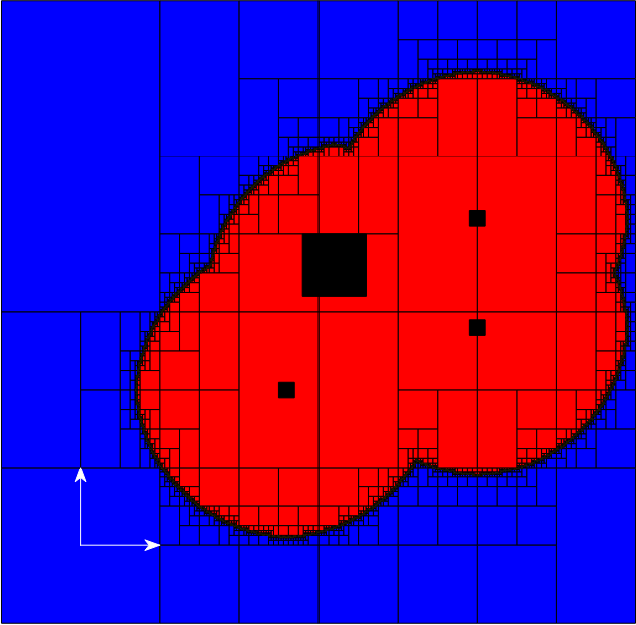
\includegraphics[scale=0.4,angle=0]{4_boat_right_border_fast_comp.png}
    \caption{Zone secured by four boat computed with algorithm ~\ref{alg:fus_boat_alg} and ~\ref{alg:one_boat_alg}.}
    \label{fig:SecureZoneFourFastBoat}
    \end{minipage}
    \begin{minipage}[b]{0.4\textwidth}
    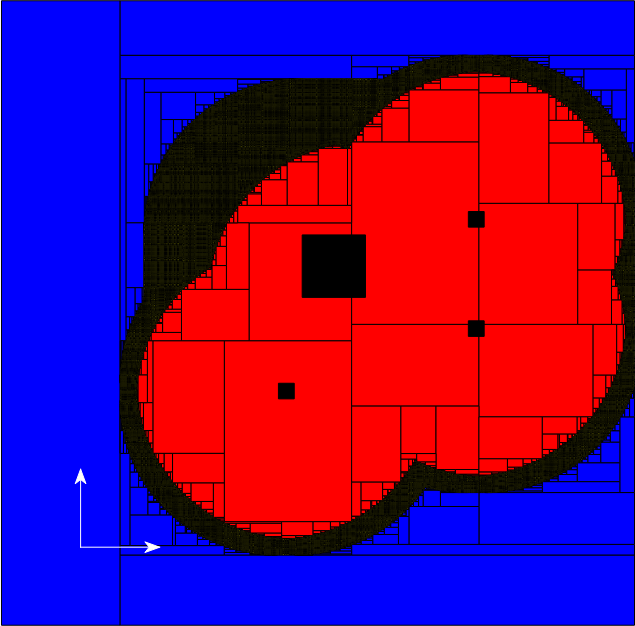
\includegraphics[scale=0.4,angle=0]{4_boat_right_border_sep_comp.png}
    \caption{Zone secured by four boat computed with separators}
    \label{fig:SecureZoneFourSepBoat}
    \end{minipage}
\end{figure}

The result in figure~\ref{fig:SecureZoneFourFastBoat} may also be obtain with the combination of separators (see figure~\ref{fig:SecureZoneFourSepBoat} but the result will be longer to get as it have to cut through the uncertain zone even if it is time consuming (and with no information gain). To demonstrate the waste of time done by the separators the figure~\ref{fig:SecureZoneFourSepBoat} has taken thirty six times the time taken to compute the figure~\ref{fig:SecureZoneFourFastBoat} (fastest computation times).